\section*{24. Stochastic Processes}\label{stochastic-processes}

\subsection*{24.1 Introduction}\label{introduction}

A \textbf{stochastic process} \(\{ X_t : t \in T \}\) is a collection of
random variables. We shall sometimes write \(X(t)\) instead of \(X_t\).
The variables \(X_t\) take values in some set \(\mathcal{X}\) called the
\textbf{state space}. The set \(T\) is called the \textbf{index set} and
for our purposes can be thought of as time. The index set can be
discrete, \(T = \{0, 1, 2, \dots \}\) or continuous \(T = [0, \infty)\)
depending on the application.

Recall that if \(X_{1}, \dots, X_{n}\) are random variables then we can
write the joint density as

\[ f(x_{1}, \dots, x_{n}) = f(x_{1}) f(x_{2} | x_{1}) \dots f(x_{n} | x_{1}, \dots, x_{n-1}) = \prod_{i=1}^{n} f(x_{i} | \text{past}_{i}) \]

where \(\text{past}_{i}\) refers to all variables before \(X_{i}\).

\subsection*{24.2 Markov Chains}\label{markov-chains}

The process \(\{ X_{n} : n \in T \}\) is a \textbf{Markov Chain} if

\[ \mathbb{P}(X_{n} = x | X_{0}, \dots, X_{n-1}) = \mathbb{P}(X_{n} = x | X_{n-1})\]

for all \(n\) and for all \(x \in \mathcal{X}\).

For a Markov chain, the joint density function can be written as

\[ f(x_{1}, \dots, x_{n}) = f(x_{1}) f(x_{2} | x_{1}) f(x_{3} | x_{2}) \dots f(x_{n} | x_{n - 1}) \]

A Markov chain can be represented by the following DAG:

\[ X_{1} \longrightarrow X_{2} \longrightarrow X_{3} \longrightarrow \cdots \longrightarrow X_{n} \longrightarrow \cdots \]

Each variable has a single parent, namely, the previous observation.

The theory of Markov chains is very rich and complex. Our goal is to
answer the following questions:

\begin{enumerate}
\def\labelenumi{\arabic{enumi}.}
\item
  When does a Markov chain ``settle down'' into some sort of
  equilibrium?
\item
  How do we estimate the parameters of a Markov chain?
\item
  How can we construct Markov chains that converge to a given
  equilibrium and why would we want to do that?
\end{enumerate}

Questions 1 and 2 will be approached this chapter, question 3 in the
next chapter.

\begin{python}
import numpy as np

def generate_random_walk(n, seed=None):
    if seed is not None:
        np.random.seed(seed)
    
    X = np.empty(n)
    X[0] = 0
    for i in range(1, n):
        X[i] = X[i - 1] + np.random.uniform(low=-1, high=1)
    
    return X

def generate_random_walk_bound(n, drift=-0.4, min_value=-10, seed=None):
    if seed is not None:
        np.random.seed(seed)
    
    X = np.empty(n)
    X[0] = 0
    for i in range(1, n):
        X[i] = max(X[i - 1] + drift, min_value) + np.random.uniform(low=-1, high=1)
    
    return X
\end{python}

\begin{python}
import matplotlib.pyplot as plt

plt.figure(figsize=(12, 8))

A = generate_random_walk(1000, seed=0)
B = generate_random_walk_bound(1000, seed=0)

ax = plt.subplot(2, 1, 1)
ax.plot(np.arange(0, len(A)), A)
ax.set_title('Does not settle into equilibrium')

ax = plt.subplot(2, 1, 2)
ax.plot(np.arange(0, len(B)), B)
ax.set_title('Does settle into equilibrium')

plt.tight_layout()
plt.show()
\end{python}

\begin{figure}[H]
\centering
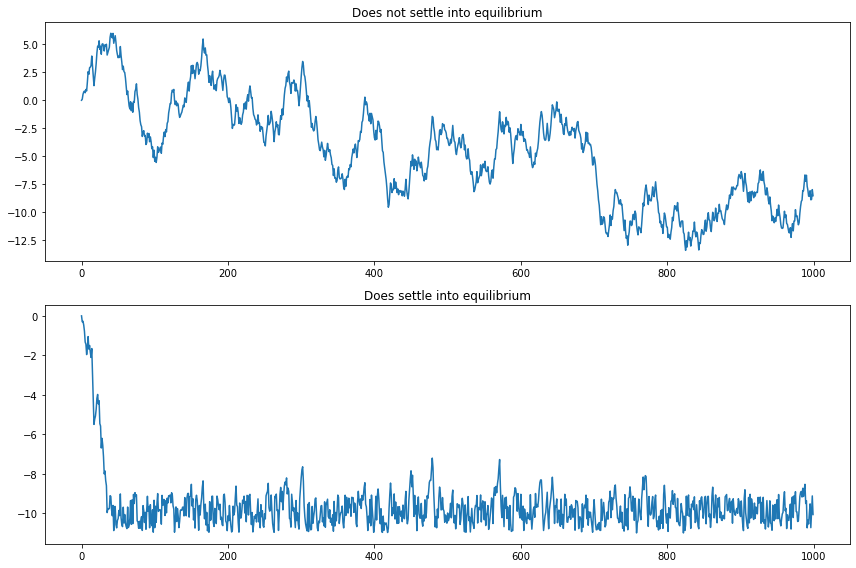
\includegraphics{Figure-24-01}
\end{figure}

\paragraph{Transition Probabilities}\label{transition-probabilities}

The key quantities of a Markov chain are the probabilities of jumping
from one state into another state.

We call

\[ \mathbb{P}(X_{n+1} = j | X_{n} = i) \]

the \textbf{transition probabilities}. If the transition probabilities
do not change with time, we say the chain is \textbf{homogeneous}. In
this case we define \(p_{ij} = \mathbb{P}(X_{n+1} = j | X_{n} = i)\). The
matrix \(P\) whose \((i, j)\) element is \(p_{ij}\) is called the
\textbf{transition matrix}.

We will only consider homogeneous chains. Notice how each \(P\) has two
properties: (i) \(p_{ij} \geq 0\) and (ii) \(\sum_{i} p_{ij} = 1\). Each
row is a probability mass function. A matrix with these properties is
called a \textbf{stochastic matrix}.

Let

\[ p_{ij}(n) = \mathbb{P}(X_{m + n} = j | X_{m} = i) \]

be the probability of going from state \(i\) to state \(j\) in \(n\)
steps. Let \(P_{n}\) be the matrix whose \((i, j)\) element is
\(p_{ij}(n)\). These are called the \textbf{\(n\)-step transition
probabilities}.

\textbf{Theorem 24.9 (The Chapman-Kolmogorov equations)}. The \(n\)-step
probabilities satisfy

\[ p_{ij}(m + n) = \sum_{k} p_{ij}(m) p_{kj}(n) \]

\textbf{Proof}. Recall that, in general,

\[ \mathbb{P}(X = x, Y = y) = \mathbb{P}(X = x) \mathbb{P}(Y = y | X = x) \]

This fact is true when conditioned in another variable,

\[ \mathbb{P}(X = x, Y = y | Z = z) = \mathbb{P}(X = x | Z = z) \mathbb{P}(Y = y | X = x, Z = z) \]

Also, recall the law of total probability:

\[ \mathbb{P}(X = x) = \sum_y \mathbb{P}(X = x, Y = y) \]

Using these facts and the Markov property we have:

\begin{align*}
p_{ij}(m + n) &= \mathbb{P}(X_{m + n} = j | X_{0} = i) \\
&= \sum_{k} \mathbb{P}(X_{m + n} = j, X_m = k | X_{0} = i) \\
&= \sum_{k} \mathbb{P}(X_{m + n} = j | X_m = k, X_{0} = i) \mathbb{P}(X_m = k | X_{0} = i) \\
&= \sum_{k} \mathbb{P}(X_{m + n} = j | X_m = k) \mathbb{P}(X_m = k | X_{0} = i) \\
&= \sum_{k} p_{ik}(m) p_{kj}(n)
\end{align*}

Note that this definition is equivalent to matrix multiplication; hence
we have shown that

\[ P_{m + n} = P_m P_{n} \]

By definition, \(P_{1} = P\). Using the above Theorem, we get

\[ P_{n} = P^{n} \equiv \underbrace{P \times P \times \cdots \times P}_{\text{multiply matrix } n \text{ times}} \]

Let \(\mu_{n} = (\mu_{n}(1), \dots, \mu_{n}(N))\) be a row vector where

\[ \mu_{n}(i) = \mathbb{P}(X_{n} = i) \]

is the marginal probability that the chain is in state \(i\) at time
\(n\). In particular, \(\mu_{0}\) is called the \textbf{initial
distribution}. To simulate a Markov chain, all you need to know is
\(\mu_{0}\) and \(P\). The simulation would look like this:

\begin{enumerate}[tightlist,label={\arabic*.}]
\item
  Draw \(X_{0} \sim \mu_{0}\). Thus, \(\mathbb{P}(X_{0} = i) = \mu_{0}(i)\).
\item
  Suppose the outcome of step 1 is \(i\). Draw \(X_{1} \sim P\). In other
  words, \(\mathbb{P}(X_{1} = j | X_{0} = i) = p_{ij}\).
\item
  Suppose the outcome of step 2 is \(j\). Draw \(X_{2} \sim P\). In other
  words, \(\mathbb{P}(X_{2} = k | X_{1} = j) = p_{jk}\).
\end{enumerate}

and so on.

It might be difficult to understand the meaning of \(\mu_{n}\). Imagine
simulating the chain many times. Collect all of the outcomes at time
\(n\) from all the chains. This histogram would look approximately like
\(\mu_{n}\). A consequence of the previous Theorem is the following:

\textbf{Lemma 24.10}. The marginal probabilities are given by

\[ \mu_{n} = \mu_{0} P^{n} \]

\textbf{Proof}.

\[ \mu_{n}(j) = \mathbb{P}(X_{n} = j) = \sum_{i} \mathbb{P}(X_{n} = j | X_{0} = i) \mathbb{P}(X_{0} = i) = \sum_{i} \mu_{0}(i) p_{ij}(n) = \mu_{0} P^{n} \]

\textbf{Summary}

\begin{enumerate}[tightlist,label={\arabic*.}]
\item
  Transition matrix: \(P(i, j) = \mathbb{P}(X_{n+1} = j | X_{n} = i)\)
\item
  \(n\)-step matrix: \(P_{n}(i, j) = \mathbb{P}(X_{m+n} = j | X_m = i)\)
\item
  \(P_{n} = P^{n}\)
\item
  Marginal probabilities: \(\mu_{n}(i) = \mathbb{P}(X_{n} = i)\)
\item
  \(\mu_{n} = \mu_{0} P^{n}\)
\end{enumerate}

\paragraph{States}\label{states}

The states of a Markov chain can be classified according to various
properties.

We say that \(i\) \textbf{reaches} \(j\) (or \(j\) is
\textbf{accessible} from \(i\)) if \(p_{ij}(n) > 0\) for some \(n\), and
we write \(i \rightarrow j\). If \(i \rightarrow j\) and
\(j \rightarrow i\) then we write \(i \leftrightarrow j\) and we say
that \(i\) and \(j\) \textbf{communicate}.

\textbf{Theorem 24.12}. The communication relation satisfies the
following properties:

\begin{enumerate}[tightlist,label={\arabic*.}]
\item
  \(i \leftrightarrow i\).
\item
  If \(i \leftrightarrow j\) then \(j \leftrightarrow i\).
\item
  If \(i \leftrightarrow j\) and \(j \leftrightarrow k\) then
  \(i \leftrightarrow k\).
\item
  The set of states \(\mathcal{X}\) can be written as a disjoint union
  of \textbf{classes}
  \(\mathcal{X} = \mathcal{X}_{1} \cup \mathcal{X}_{2} \cup \cdots\) where
  two states \(i\) and \(j\) communicate with each other if and only if
  they are in the same class.
\end{enumerate}

If all states communicate with each other then the chain is called
\textbf{irreducible}. A set of states is \textbf{closed} if once you
enter that set states you never leave. A closet set consisting of a
single state is called an \textbf{absorbing state}.

Suppose we start a chain in state \(i\). Will the chain ever return to
state \(i\)? If so, that state is called persistent or recurrent.

State \(i\) is \textbf{recurrent} or \textbf{persistent} if

\[ \mathbb{P}(X_{n} = i \text{ for some } n \geq 1 | X_{0} = i) = 1 \]

Otherwise, state \(i\) is \textbf{transient}.

\textbf{Theorem 24.15}. A state \(i\) is recurrent if and only if

\[ \sum_{n} p_{ii}(n) = \infty \]

A state \(i\) is transient if and only if

\[ \sum_{n} p_{ii}(n) < \infty \]

\textbf{Proof}. Define

\[ 
I_{n} = \begin{cases}
1 & \text{if } X_{n} = i \\
0 & \text{if } X_{n} \neq i
\end{cases}
\]

The number of times that the chain is in state \(i\) is
\(Y = \sum_{n=0}^{\infty} I_{n}\). The mean of \(Y\), given that the chain
starts in state \(i\), is

\begin{align*}
\mathbb{E}(Y | X_{0} = i) &= \sum_{n=0}^{\infty} \mathbb{E}(I_{n} | X_{0} = i) \\
&= \sum_{n=0}^{\infty} \mathbb{P}(X_{n} = i | X_{0} = i) \\
&= \sum_{n=0}^{\infty} p_{ii}(n)
\end{align*}

Define
\(a_{i} = \mathbb{P}(X_{n} = i \text{ for some } n \geq 1 | X_{0} = i)\). If
\(i\) is recurrent, \(a_{i} = 1\). Thus, the chain will eventually return
to \(i\). Once it does, we argue again that since \(a_{i} = 1\), the chain
will return to state \(i\) again. By repeating this argument, we
conclude that \(\mathbb{E}(Y | X_{0} = i) = \infty\).

If \(i\) is transient, then \(a_{i} < 1\). When the chain is in state
\(i\), there is a probability \(1 - a_{i} > 0\) that it will never return
to state \(i\). Thus, the probability that the chain is in state \(i\)
exactly \(n\) times is \(a_{i}^{n - 1}(1 - a_{i})\). This is a geometric
distribution that has finite mean.

\textbf{Theorem 24.16}. Facts about recurrence:

\begin{enumerate}[tightlist,label={\arabic*.}]
\item
  If a state \(i\) is recurrent and \(i \leftrightarrow j\) then \(j\)
  is recurrent.
\item
  If a state \(i\) is transient and \(i \leftrightarrow j\) then \(j\)
  is transient.
\item
  A finite Markov chain must have at least one recurrent state.
\item
  The states of a finite, irreducible Markov chain are all recurrent.
\end{enumerate}

\textbf{Theorem 24.17 (Decomposition Theorem)}. The state space
\(\mathcal{X}\) can be written as the disjoint union

\[ \mathcal{X} = \mathcal{X}_{T} \cup \mathcal{X}_{1} \cup \mathcal{X}_{2} \cup \cdots \]

where the \(\mathcal{X}_T\) are the transient states and each
\(\mathcal{X}_{i}\) is a closed, irreducible set of recurrent states.

\paragraph{Convergence of Markov Chains}\label{convergence-of-markov-chains}

Suppose that \(X_{0} = i\). Define the \textbf{recurrence time}

\[ T_{ij} = \min \{ n > 0 : X_{n} = j \} \]

assuming \(X_{n}\) ever returns to the state \(i\), otherwise define
\(T_{ij} = \infty\). The \textbf{mean recurrence time} of a recurrent
state \(i\) is

\[ m_{i} = \mathbb{E}(T_{ii}) = \sum_{n} n f_{ii}(n) \]

where

\[ f_{ij}(n) = \mathbb{P}(X_{1} \neq j, X_{2} \neq j, \dots, X_{n-1} \neq j, X_{n} \neq j | X_{0} = i) \]

A recurrent state is \textbf{null} if \(m_{i} = \infty\), otherwise it is
called \textbf{non-null} or \textbf{positive}.

\textbf{Lemma 24.18}. If a state is null and recurrent, then
\(p_{ii}^{n} \rightarrow 0\).

\textbf{Lemma 24.19}. In a finite state Markov chain, all recurrent
states are positive.

Consider a three state chain with transition matrix

\[
\begin{bmatrix}
0 & 1 & 0 \\
0 & 0 & 1 \\
1 & 0 & 0
\end{bmatrix}
\]

Suppose we start the chain in state 1. Then we will be in state 3 at
times \(3, 6, 9, \dots\). This is an example of a periodic chain.
Formally, the \textbf{period} of state \(i\) is \(d\) is
\(p_{ii}(n) = 0\) whenever \(n\) is not divisible by \(d\) and \(d\) is
the largest integer with this property. Thus,
\(d = \text{gcd} \{ n : p_{ii}(n) = 0 \}\), where gcd means ``greatest
common divisor''. State \(i\) is \textbf{periodic} if \(d(i) > 1\) and
\textbf{aperiodic} if \(d(i) = 1\).

\textbf{Lemma 24.20}. If a state \(i\) has period \(d\) and
\(i \leftrightarrow j\) then \(j\) has period \(d\).

A state is \textbf{ergodic} if it is recurrent, non-null and aperiodic.
A chain is ergodic if all its states are ergodic.

Let \(\pi = (\pi_{i} : i \in \mathcal{X})\) be a vector of non-negative
numbers that sum to one. Thus \(\pi\) can be thought of as a probability
mass function.

We say that \(\pi\) is a \textbf{stationary} (or \textbf{invariant})
distribution if \(\pi = \pi P\).

Here is the intuition. Draw \(X_{0}\) from distribution \(\pi\) and
suppose that \(\pi\) is a stationary distribution. Now draw \(X_{1}\)
according to the transition probability of the chain. The distribution
of \(X_{1}\) is then \(\mu_{1} = \mu_{0} P = \pi P = \pi\). Continuing this
way, the distribution of \(X_{n}\) is
\(\mu_{n} = \mu_{0} P^{n} = \pi P^{n} = \pi\). In other words: if at any time
the chain has distribution \(\pi\), then it will continue to have
distribution \(\pi\) forever.

We say that a chain has \textbf{limiting distribution} if

\[ P^{n} \rightarrow \begin{bmatrix}
\pi \\ \pi \\ \vdots \\ \pi
\end{bmatrix}\]

for some \(\pi\). In other words,
\(\pi_{j} = \lim_{n \rightarrow \infty} P_{ij}^{n}\) exists and is
independent of \(i\).

\textbf{Theorem 24.24}. An irreducible, ergodic Markov chain has a
unique stationary distribution \(\pi\). The limiting distribution exists
and is equal to \(\pi\). If \(g\) is any bounded function, then, with
probabiity 1,

\[ \lim_{N \rightarrow \infty} \frac{1}{N} \sum_{n=1}^N g(X_{n}) = \mathbb{E}_\pi(g) \equiv \sum_{j} g(j) \pi_{j} \]

The last statement of the Theorem is the law of large numbers for Markov
chains. It says that sample averages converge to their expectations.
Finally, there is a special condition which will be useful later. We say
that \(\pi\) satisfies \textbf{detailed balance} if

\[ \pi_{i} p_{ij} = p_{ji} \pi_{j} \]

Detailed balance guarantees that \(\pi\) is a stationary distribution.

\textbf{Theorem 24.25}. If \(\pi\) satisfies detailed balance then
\(\pi\) is a stationary distribution.

\textbf{Proof}. We need to show that \(\pi P = \pi\). The \(j\)-th
element of \(\pi P\) is
\(\sum_{i} \pi_{i} p_{ij} = \sum_{i} p_{ji}\pi_{j} = \pi_{j} \sum_{i} p_{ji} = \pi_{j}\).

The importance of detailed balance will become clear when we discuss
Markov chain Monte Carlo methods.

\textbf{Warning}: Just because a chain has a stationary distribution
does not mean it converges.

\paragraph{Inference for Markov Chains}\label{inference-for-markov-chains}

Consider a chain with finite state space $\mathcal{X} = \{ 1, 2, \dots,
N \} $. Suppose we observe \(n\) observations \(X_{1}, \dots, X_{n}\) from
this chain. The unknown parameters of a Markov chain are the initial
probabilities \(\mu_{0} = (\mu_{0}(1), \mu_{0}(2), \dots)\) and the elements
of the transition matrix \(P\). Each row of \(P\) is a multinomial
distribution, so we are essentially estimating \(N\) distributions (plus
the initial probabilities). Let \(n_{ij}\) be the observed number of
transitions from state \(i\) to state \(j\). The likelihood function is

\[ \mathcal{L}(\mu_{0}, P) = \mu_{0}(x_{0}) \prod_{r=1}^{n} p_{X_{r - 1}, X_r} = \mu_{0}(x_{0}) \prod_{i=1}^N \prod_{j=1}^N p_{ij}^{n_{i}j} \]

There is only one observation on \(\mu_{0}\) so we cannot estimate that.
Rather, we focus on estimating \(P\). The MLE is obtained by maximizing
the likelihood subject to the constraint that the elements are
non-negative and the rows sum to 1. The solution is

\[ \hat{p}_{ij} = \frac{n_{ij}}{n_{i}} \]

where \(n_{i} = \sum_{j=1}^N n_{ij}\). Here we are assuming that
\(n_{i} > 0\). If not, we set \(\hat{p}_{ij} = 0\) by convention.

\textbf{Theorem 24.30 (Consistency and Asymptotic Normality of the
MLE)}. Assume that the chain is ergodic. Let \(\hat{p}_{ij}(n)\) denote
the MLE after \(n\) observations. Then
\(\hat{p}_{ij}(n) \xrightarrow{\text{P}} p_{ij}\). Also,

\[ \left[ \sqrt{N_{i}(n)} (\hat{p}_{ij} - p_{ij})  \right] \leadsto N(0, \Sigma) \]

where the left hand side is a matrix, $ N\_{i}(n) = \sum\_\{r=1\}^{n}
I(X\_r = i)$ is the count of observations at state \(i\) up to time
\(n\), and the covariance matrix \(\Sigma\) is a \(t \times t\) matrix,
where \(t\) is the number of transitions from state \(i\) to \(j\), with
elements

\[ 
\Sigma_{ij, k\ell} = \begin{cases}
p_{ij}(1 - p_{ij}) &\text{if } (i, j) = (k, \ell) \\
-p_{ij} p_{i\ell} &\text{if } i = k, j \neq \ell \\
0 &\text{otherwise}
\end{cases}
\]

\subsection*{24.3 Poisson Process}\label{poisson-process}

As the name suggests, the Poisson process is intimately related to the
Poisson distribution. First review the Poisson distribution.

Recall that \(X\) has a Poisson distribution with parameter \(\lambda\),
written \(X \sim \text{Poisson}(\lambda)\), if

\[ \mathbb{P}(X = x) \equiv p(x; \lambda) = \frac{e^{-\lambda} \lambda^x}{x!}, \quad = 0, 1, 2, \dots \]

Also recall that: - \(X \sim \text{Poisson}(\lambda)\) distribution has
mean \(\mathbb{E}(X) = \lambda\) and variance
\(\mathbb{V}(X) = \lambda\). - If \(X \sim \text{Poisson}(\lambda)\),
\(Y \sim \text{Poisson}(\nu)\) and \(X\) and \(Y\) are independent, then
\(X + Y \sim \text{Poisson}(\lambda + \nu)\). - If
\(N \sim \text{Poisson}(\lambda)\) and
\(Y | N = n \sim \text{Binomial}(n, p)\) then the marginal distribution
of \(Y\) is \(Y \sim \text{Poisson}(\lambda p)\).

Now we describe the Poisson process. Imagine that whenever an event
occurs you record its timestamp. Let \(X_t\) be the number of events
that occured up until time \(t\). Then,
\(\{ X_t : t \in [0, \infty) \}\) is a stochastic process with state
space \(\mathcal{X} = \{ 0, 1, 2, \dots \}\). A process of this form is
called a \textbf{counting process}.

In what follows, we will sometimes write \(X(t)\) instead of \(X_t\).
Also, we will need little-o notation: write \(f(h) = o(h)\) if
\(f(h) / h \rightarrow 0\) as \(h \rightarrow 0\). This means that
\(f(h)\) is smaller than \(h\) when \(h\) is close to 0. For example,
\(h^{2} = o(h)\).

A \textbf{Poisson process} is a stochastic process
\(\{ X_t : t \in [0, \infty) \}\) with state space
\(\mathcal{X} = \{ 0, 1, 2, \dots \}\) such that

\begin{enumerate}[tightlist,label={\arabic*.}]
\item
  \(X(0) = 0\)
\item
  For any increasing times \(0 = t_{0} < t_{1} < t_{2} < \dots < t_{n}\), the
  count increments
\end{enumerate}

\[ X(t_{1}) - X(t_{0}), X(t_{2}) - X(t_{1}), \dots, X(t_{n}) - X(t_{n - 1})\]

are independent.

\begin{enumerate}[tightlist,label={\arabic*.},resume]
\item
  There is a function \(\lambda(t)\) such that
\end{enumerate}

\begin{align*}
\mathbb{P}\left(X(t + h) - X(t) = 1\right) &= \lambda(t)h + o(h) \\
\mathbb{P}\left(X(t + h) - X(t) \geq 2\right) &= o(h)
\end{align*}

We call \(\lambda(t)\) the \textbf{intensity function}.

\textbf{Theorem 24.32}. If \(X_t\) is a Poisson process with intensity
function \(\lambda(t)\), then

\[ X(s + t) - X(s) \sim \text{Poisson}\left( m(s + t) - m(s) \right) \]

where

\[ m(t) = \int_{0}^t \lambda(s) ds \]

In particular, \(X(t) \sim \text{Poisson}(m(t))\). Hence,
\(\mathbb{E}(X(t)) = m(t)\) and \(\mathbb{V}(X(t)) = m(t)\).

A Poisson process with constant intensity function
\(\lambda(t) \equiv \lambda\) for some \(\lambda > 0\) is called a
\textbf{homogeneous Poisson process} with rate \(\lambda\). In this
case,

\[ X(t) \sim \text{Poisson}(\lambda t) \]

Let \(X(t)\)be a homogeneous Poisson process with rate \(\lambda\). Let
\(W_{n}\) be the time at which the \(n\)-th event occurs and set
\(W_{0} = 0\). The random variables \(W_{0}, W_{1}, \dots\) are called
\textbf{waiting times}. Let \(S_{n} = W_{n + 1} - W_{n}\). Then
\(S_{0}, S_{1}, \dots\) are called \textbf{sojourn times} or
\textbf{interarrival times}.

\textbf{Theorem 24.34}. The sojourn times \(S_{0}, S_{1}, \dots\) are IID
random variables. Their distribution is exponential with mean
\(1 / \lambda\), that is, they have density

\[ f(s) = \lambda e^{-\lambda s}, \quad s \geq 0 \]

The waiting time has distribution
\(W_{n} \sim \text{Gamma}(n, 1 / \lambda)\), that is, it has density

\[ f(w) = \frac{1}{\Gamma(n)} \lambda^{n} w^{n - 1}e^{-\lambda t} \]

Hence, \(\mathbb{E}(W_{n}) = n / \lambda\) and
\(\mathbb{V}(W_{n}) = n / \lambda^{2}\).

\textbf{Proof}. First, we have

\[ \mathbb{P}(S_{1} > t) = \mathbb{P}(X(t) = 0) = e^{-\lambda t}\]

which shows that the CDF for \(S_{1}\) is \(1 - e^{-\lambda t}\). This
shows the result for \(S_{1}\). Now,

\begin{align*}
\mathbb{P}(S_{2} | t | S_{1} = s) &= \mathbb{P}\left(\text{no events in } (s, s+t] | S_{1} = s\right) \\
&= \mathbb{P}\left(\text{no events in } (s, s+t]\right) \quad \text{(increments are independent)} \\
&= e^{-\lambda t}
\end{align*}

Hence, \(S_{2}\) has an exponential distribution and is independent of
\(S_{1}\). The result follows by repeating the argument. The result for
\(W_{n}\) follows since a sum of exponentials has a Gamma distribution.

\subsection*{24.6 Exercises}

\textbf{Exercise 24.6.1} Let \(X_{0}, X_{1}, \dots\) be a Markov chain with
states \(\{ 0, 1, 2 \}\) and transition matrix

\[ P = \begin{bmatrix}
0.1 & 0.2 & 0.7 \\
0.9 & 0.1 & 0.0 \\
0.1 & 0.8 & 0.1
\end{bmatrix}\]

Assume that \(\mu_{0} = (0.3, 0.4, 0.3)\). Find
\(\mathbb{P}(X_{0} = 0, X_{1} = 1, X_{2} = 2)\) and
\(\mathbb{P}(X_{0} = 0, X_{1} = 1, X_{2} = 1)\).

\textbf{Solution}.

We have:

\begin{align*}
\mathbb{P}(X_{0} = 0, X_{1} = 1, X_{2} = 2) &= \mathbb{P}(X_{0} = 0) \mathbb{P}(X_{1} = 1 | X_{0} = 0) \mathbb{P}(X_{2} = 2 | X_{1} = 1) \\
&= \mu_{0}(1) P_{12} P_{23} \\
& = 0.3 \cdot 0.2 \cdot 0.0 \\
& = 0
\end{align*}

which can also be seen since there is no probability for a transition
from state 1 to state 2 (the corresponding value in the \(P\) matrix is
zero).

We also have:

\begin{align*}
\mathbb{P}(X_{0} = 0, X_{1} = 1, X_{2} = 2) &= \mathbb{P}(X_{0} = 0) \mathbb{P}(X_{1} = 1 | X_{0} = 0) \mathbb{P}(X_{2} = 1 | X_{1} = 1) \\
&= \mu_{0}(1) P_{12} P_{22} \\
& = 0.3 \cdot 0.2 \cdot 0.1 \\
& = 0.006
\end{align*}

\textbf{Exercise 24.6.2}. Let \(Y_{1}, Y_{2}, \dots\) be a sequence of iid
observations such that \(\mathbb{P}(Y = 0) = 0.1\),
\(\mathbb{P}(Y = 1) = 0.3\), \(\mathbb{P}(Y = 2) = 0.2\),
\(\mathbb{P}(Y = 3) = 0.4\). Let \(X_{0} = 0\) and let

\[ X_{n} = \max \{ Y_{1}, \dots, Y_{n} \} \]

Show that \(X_{0}, X_{1}, \dots\) is a Markov chain and find the transition
matrix.

\textbf{Solution}. By definition,

\[ X_{n + 1} = \max \{Y_{1}, \dots, Y_{n+1} \} = \max \{ X_{n}, Y_{n + 1} \} \]

so \(X_{n + 1}\) is defined based only on its predecessor and on a IID
variable \(Y_{n+1} \sim Y\). Thus:

\[ \mathbb{P}(X_{n + 1} = j | X_{n} = i) = \begin{cases}
\frac{\mathbb{P}(Y = j)}{\sum_{k \geq i} \mathbb{P}(Y = k)} & \text{if } j \geq i \\
0 &\text{if } j < i
\end{cases} \]

This, paired with a state space $\mathcal{X} = \{ 0, 1, 2, 3 \} $ and
initial probabilities \(\mu_{0} = (1, 0, 0, 0)\), defines a Markov chain
for the \(X_{i}\)s. The explicit transition matrix is:

\[ P = \begin{bmatrix}
1/10 & 3/10 & 1/5 & 2/5 \\
0   & 1/3 & 2/9 & 4/9 \\
0   & 0   & 1/3 & 2/3 \\
0   & 0   & 0   & 1
\end{bmatrix}\]

\textbf{Exercise 24.6.3}. Consider a two state Markov chain with states
\(\mathcal{X} = \{ 1, 2 \}\) and transition matrix

\[ P = \begin{bmatrix}
1 - a & a \\
b & 1 - b
\end{bmatrix} \]

where \(0 < a < 1\) and \(0 < b < 1\). Prove that

\[ \lim_{n \rightarrow \infty} P^{n} = \begin{bmatrix}
\frac{b}{a + b} & \frac{a}{a + b} \\
\frac{b}{a + b} & \frac{a}{a + b}
\end{bmatrix} \]

\textbf{Solution}. Note that the Markov chain is irreducible and
ergodic, given the bounds on \(a\) and \(b\). Note also that it has a
stationary distribution

\[ \pi = \left( \frac{b}{a + b}, \frac{a}{a + b} \right) \]

since \(\pi = \pi P\):

\begin{align*}
\pi P &= 
\begin{bmatrix} 
\frac{b}{a + b} & \frac{a}{a + b}
\end{bmatrix} \begin{bmatrix}
1 - a & a \\
b & 1 - b
\end{bmatrix} \\
&= \frac{1}{a + b} \begin{bmatrix}
 b (1 - a) + ab &
 ab + (1 - b) a 
\end{bmatrix} \\
&= \begin{bmatrix} \frac{b}{a + b} & \frac{a}{a + b} \end{bmatrix}\\
&= \pi
\end{align*}

By Theorem 24.24, the limit of \(P^{n}\) is as given,

\[ \lim_{n \rightarrow \infty} P^{n} = 
\begin{bmatrix}
\pi \\ \pi
\end{bmatrix}
=
\begin{bmatrix}
\frac{b}{a + b} & \frac{a}{a + b} \\
\frac{b}{a + b} & \frac{a}{a + b}
\end{bmatrix} \]

\textbf{Exercise 24.6.4}. Consider the chain from question 3 and set
\(a = .1\) and \(b = .3\). Simulate the chain. Let

\[
\hat{p}_{n}(1) = \frac{1}{n} \sum_{i=1}^{n} I(X_{i} = 1)
\quad \text{and} \quad
\hat{p}_{n}(2) = \frac{1}{n} \sum_{i=1}^{n} I(X_{i} = 2)
\]

be the proportion of times the chain is in state 1 and state 2. Plot
\(\hat{p}_{n}(1)\) and \(\hat{p}_{n}(2)\) versus \(n\) and verify that they
converge to the values predicted from the answer in the previous
question.

\textbf{Solution}.

\begin{python}
import numpy as np

a, b = 0.1, 0.3
P = np.array([[1 - a, a], [b, 1 - b]])
\end{python}

\begin{python}
# Do a *single* simulation starting from, say, state 1

def generate_series(n, seed=None, initial_state=1):
    if seed is not None:
        np.random.seed(0)

    random_values = np.random.uniform(low=0, high=1, size=n)

    X = np.empty(n, dtype=int)
    X[0] = initial_state
    for i in range(1, n):
        X[i] = 1 if random_values[i] < P[X[i - 1] - 1, 0] else 2
        
    return X

n = 10000
X = generate_series(n, seed=0)
p1 = np.cumsum(X == 1) / np.arange(1, n + 1)
p2 = np.cumsum(X == 2) / np.arange(1, n + 1)
\end{python}

\begin{python}
import matplotlib.pyplot as plt

plt.figure(figsize=(12, 8))
plt.plot(np.arange(1, n+1), p1, label=r'$\hat{p}_{n}(1)$')
plt.plot(np.arange(1, n+1), p2, label=r'$\hat{p}_{n}(2)$')
plt.legend()
plt.show()
\end{python}s

\begin{figure}[H]
\centering
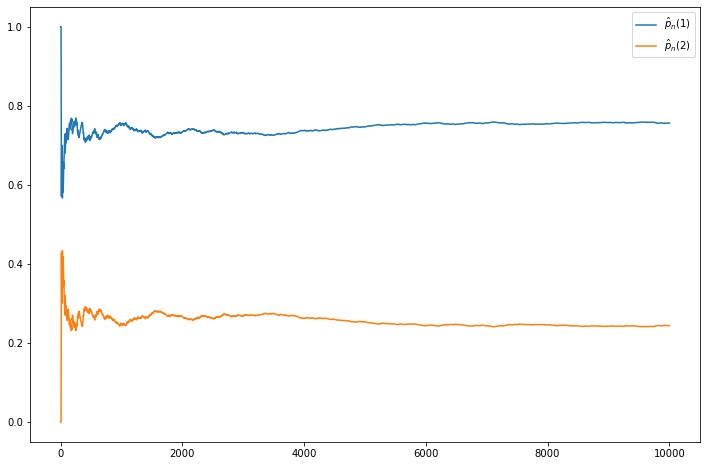
\includegraphics{Figure-24-02}
\end{figure}

Note that the values do converge to \(\pi = (0.75, 0.25)\).

\textbf{Exercise 24.6.5}. An important Markov chain is the
\textbf{branching process} which is used in biology, genetics, nuclear
physics and many other fields. Suppose that an animal has \(Y\)
children. Let \(p_{k} = \mathbb{P}(Y = k)\). Hence \(p_{k} \geq 0\) for all
\(k\) and \(\sum_{k = 0}^{\infty} p_{k} = 1\). Assume each animal has the
same lifespan and that they produce offspring according to the
distribution \(p_{k}\). Let \(X_{n}\) be the number of animals in the
\(n\)-th generation. Let \(Y_{1}^{(n)}, \dots, Y_{X_{n}}^{(n)}\) be the
offspring produced in the \(n\)-th generation. Note that

\[ X_{n+1} = Y_{1}^{(n)} + \dots + Y_{X_{n}}^{(n)}\]

Let \(\mu = \mathbb{E}(Y)\) and \(\sigma^{2} = \mathbb{V}(Y)\). Assume
throughout this question that \(X_{0} = 1\). Let
\(M(n) = \mathbb{E}(X_{n})\) and \(V(n) = \mathbb{V}(X_{n})\).

\textbf{(a)} Show that \(M(n + 1) = \mu M(n)\) and that $V(n + 1) =
\sigma^{2} M(n) + \mu^{2} V(n) $.

\textbf{(b)} Show that \(M(n) = \mu^{n}\) and that
\(V(n) = \sigma^{2} \mu^{n-1} (1 + \mu + \dots + \mu^{n - 1})\).

\textbf{(c)} What happens to the variance if \(\mu > 1\)? What happens
to the variance if \(\mu = 1\)? What happens to the variance if
\(\mu < 1\)?

\textbf{(d)} The population goes extinct if \(X_{n} = 0\) for some \(n\).
Let us thus define the extinction time \(N\) by

\[ N = \min \{ n : X_{n} = 0 \} \]

Let \(F(n) = \mathbb{P}(N \leq n)\) be the CDF of the random variable
\(N\). Show that

\[ F(n) = \sum_{k=0}^{\infty} p_{k} \left( F(n - 1) \right)^{k}, \quad n = 1, 2, \dots \]

Hint: note that the event \(\{ N \leq n \}\) is the same event as
\(\{ X_{n} = 0 \}\). Thus \(\mathbb{P}(N \leq n) = \mathbb{P}(X_{n} = 0)\).
Let \(k\) be the number of offspring of the original event. The
population becomes extinct at time \(n\) if and only if each of the
\(k\) sub-populations generated from the \(k\) offspring goes extinct in
\(n - 1\) generations.

\textbf{(e)} Suppose that \(p_{0} = 1/4\), \(p_{1} = 1/2\), \(p_{2} = 1/4\).
Use the formula from (d) to compute the CDF \(F(n)\).

\textbf{Solution}.

\textbf{(a)} We have:

\[ M(n + 1) = \mathbb{E}[X_{n + 1}] = \mathbb{E}\left[ \sum_{i = 1}^{X_{n}} Y_{i}^{(n)} \right] = \mathbb{E}\left[ \sum_{i = 1}^{X_{n}} \mathbb{E}[Y_{i}^{(n)}] \right] = \mathbb{E}\left[ \sum_{i = 1}^{X_{n}} \mu \right]  = \mu \mathbb{E}[X_{n}] = \mu M(n)\]

We also have:

\begin{align*}
V(n + 1) &= \mathbb{V}[X_{n + 1}] = \mathbb{E}[X_{n + 1}^{2}] - \mathbb{E}[X_{n + 1}]^{2} \\
&= \mathbb{E}\left[\left( \sum_{i = 1}^{X_{n}} Y_{i}^{(n)} \right)^{2}\right] - \mu^{2} M(n)^{2} \\
&= \mathbb{E}\left[ \sum_{i = 1}^{X_{n}} \left( Y_{i}^{(n)} \right)^{2} + \sum_{i = 1}^{X_{n}} \sum_{j = 1, j \neq i}^{X_{n}} Y_{i}^{(n)} Y_{j}^{(n)} \right] - \mu^{2} M(n)^{2} \\
&= \mathbb{E}\left[ \sum_{i = 1}^{X_{n}} \mathbb{E}\left[\left( Y_{i}^{(n)} \right)^{2}\right] + \sum_{i = 1}^{X_{n}} \sum_{j = 1, j \neq i}^{X_{n}} \mathbb{E}\left[ Y_{i}^{(n)} Y_{j}^{(n)} \right] \right] - \mu^{2} M(n)^{2} \\
&= \mathbb{E}\left[ \sum_{i = 1}^{X_{n}} \left( \mathbb{V}[Y_{i}^{(n)}] +  \mathbb{E}\left[ Y_{i}^{(n)} \right]^{2} \right) + \sum_{i = 1}^{X_{n}} \sum_{j = 1, j \neq i}^{X_{n}} \mathbb{E}\left[ Y_{i}^{(n)} \right] \mathbb{E} \left[ Y_{j}^{(n)} \right] \right] - \mu^{2} M(n)^{2} \\
&= \mathbb{E}\left[ \sum_{i = 1}^{X_{n}} \left( \sigma^{2} + \mu^{2} \right) + \sum_{i = 1}^{X_{n}} \sum_{j = 1, j \neq i}^{X_{n}} \mu^{2} \right] - \mu^{2} M(n)^{2} \\
&= \mathbb{E} \left[ X_{n} (\sigma^{2} + \mu^{2}) + X_{n} (X_{n} - 1) \mu^{2} \right] - \mu^{2} M(n)^{2} \\
&= \mathbb{E} \left[ X_{n} \sigma^{2} + X_{n}^{2} \mu^{2} \right] - \mu^{2} M(n)^{2} \\
&= \sigma^{2} \mathbb{E} [ X_{n} ] + \mu^{2} \mathbb{E} [ X_{n}^{2} ] - \mu^{2} M(n)^{2} \\
&= \sigma^{2} M(n) + \mu^{2} (V(n) + M(n)^{2}) - \mu^{2} M(n)^{2} \\
&= \sigma^{2} M(n) + \mu^{2} V(n)
\end{align*}

\textbf{(b)}

Since the initial population is 1, \(M(0) = 1\); since
\(M(n + 1) = \mu M(n)\), it follows by induction that \(M(n) = \mu^{n}\).

Now, we also have that the initial population is known, so \(V(0) = 0\).
By induction,

\begin{align*}
V(n + 1) &= \sigma^{2} M(n) + \mu^{2} V(n) \\
&= \sigma^{2} \mu^{n} + \mu^{2} \left( \sigma^{2} \mu^{n - 1} \left( 1 + \mu + \dots + \mu^{n - 1}\right) \right) \\
&= \sigma^{2} \mu^{n} \left(1 + \mu \left( 1 + \mu + \dots + \mu^{n - 1} \right) \right) \\
&= \sigma^{2} \mu^{n} \left(1 + \mu + \dots + \mu^{n} \right)
\end{align*}

\textbf{(c)} If \(\mu \neq 1\), we can add up the geometric sum and
write

\[ V(n) = \sigma^{2} \mu^{n} \frac{1 - \mu^{n}}{1 - \mu}\]

\begin{itemize}[tightlist]
\item
  For \(\mu > 1\), \(V(n)\) grows exponentially.\\
\item
  For \(\mu < 1\), \(V(n)\) converges to 0.\\
\item
  For \(\mu = 1\), we have \(V(n) = n \sigma^{2}\), which grows linearly.
\end{itemize}

\textbf{(d)} Following the reasoning in the hint,

\begin{align*}
F(n) &= \mathbb{P}(N \leq n) = \mathbb{P}(X_{n} = 0) \\
&= \sum_{k=0}^{\infty} \mathbb{P}(X_{n} = 0 | X_{1} = k) \mathbb{P}(X_{1} = k) \\
&= \sum_{k=0}^{\infty} \mathbb{P}(Y_{i}^{(n - 1)} = 0 \text{ for all } i | X_{1} = k) \mathbb{P}(X_{1} = k) \\
&= \sum_{k=0}^{\infty} \left( \prod_{i=1}^{k} \mathbb{P}(Y_{i}^{(n - 1)} = 0 | X_{1} = k) \right) \mathbb{P}(X_{1} = k) \\
&= \sum_{k=0}^{\infty} \left( \prod_{i=1}^{k} F(n-1) \right) p_{k} \\
&= \sum_{k=0}^{\infty} p_{k} \left( F(n - 1)\right)^{k}
\end{align*}

\textbf{(e)} The recurrence formula is:

\[ F(n + 1) = p_{0} + p_{1} F(n) + p_{2} F(n)^{2} = \frac{1}{4} + \frac{1}{2} F(n) + \frac{1}{4} F(n)^{2} = \frac{1}{4} (F(n) + 1)^{2}\]

with initial value \(F(0) = 0\) (since we start with a non-extinct
population).

\begin{python}
import numpy as np

N = 1000
F = np.empty(N)

F[0] = 0
for n in range(1, N):
    F[n] = (F[n - 1] + 1)**2 / 4
\end{python}

\begin{python}
import matplotlib.pyplot as plt
%matplotlib inline

plt.figure(figsize=(12, 8))
plt.plot(np.arange(1, N + 1), F)
plt.xlabel('N')
plt.ylabel('F(N)')
plt.xscale('log')
plt.show()
\end{python}

\begin{figure}[H]
\centering
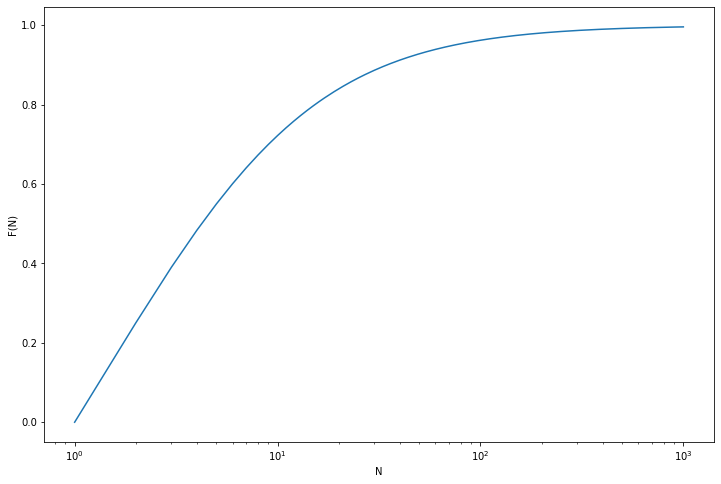
\includegraphics{Figure-24-03}
\end{figure}

\textbf{Exercise 24.6.6}. Let

\[ P = \begin{bmatrix}
0.40 & 0.50 & 0.10 \\
0.05 & 0.70 & 0.25 \\
0.05 & 0.50 & 0.45
\end{bmatrix}\]

Find the stationary distribution \(\pi\).

\textbf{Solution}. The stationary distribution \(\pi\) satisfies
\(\pi = \pi P\), so it is a (normalized) left eigenvector of \(P\), or a
right eigenvector of \(P^T\).

\begin{python}
import numpy as np
from numpy.linalg import eig

P = np.array([[0.4, 0.5, 0.1], [0.05, 0.7, 0.25], [0.05, 0.5, 0.45]])
\end{python}

\begin{python}
w, v = eig(P.T)
pi = v[:, 0]
print(pi)
\end{python}

\begin{console}
[0.11041049 0.89708523 0.42784065]
\end{console}

\begin{python}
print(pi @ P)
\end{python}

\begin{console}
[0.11041049 0.89708523 0.42784065]
\end{console}

\textbf{Exercise 24.6.7}. Show that if \(i\) is a recurrent state and
\(i \leftrightarrow j\), then \(j\) is a recurrent state.

\textbf{Solution}.

Since \(i\) is recurrent, \(\sum_{n} p_{ii}(n) = \infty\). But

\[\sum_{n} p_{jj}(n) \geq \sum_{a, b, c} p_{ji}(a) p_{ii}(b) p_{ij}(c) \geq \sum_b p_{ji}(a') p_{ii}(b) p_{ij}(c')\]

for some \(a'\) such that \(p_{ji}(a') > 0\) (which exists because
\(j \rightarrow i\)) and some \(c'\) such that \(p_{ij}(c') > 0\) (which
exists because \(i \rightarrow j\)). Then this sum is lower bounded by

\[\frac{1}{p_{ji}(a') p_{ij}(c')} \sum_b p_{ii}(b)\]

which diverges because \(\sum_{n} p_{ii}(n) = \infty\), so \(j\) must be a
recurrent state.

\textbf{Exercise 24.6.8}. Let

\[ P = \begin{bmatrix}
1/3 & 0   & 1/3 & 0 & 0 & 1/3 \\
1/2 & 1/4 & 1/4 & 0 & 0 & 0   \\
0   & 0   & 0   & 0 & 1 & 0   \\
1/4 & 1/4 & 1/4 & 0 & 0 & 1/4 \\
0   & 0   & 1   & 0 & 0 & 0   \\
0   & 0   & 0   & 0 & 0 & 1
\end{bmatrix}\]

Which states are transient? Which states are recurrent?

\textbf{Solution}.

\begin{python}
from graphviz import Digraph

d = Digraph()

d.edge('1', '1', label='1/3')
d.edge('1', '3', label='1/3')
d.edge('1', '6', label='1/3')

d.edge('2', '1', label='1/2')
d.edge('2', '2', label='1/4')
d.edge('2', '3', label='1/4')

d.edge('3', '5', label='1')

d.edge('4', '1', label='1/4')
d.edge('4', '2', label='1/4')
d.edge('4', '3', label='1/4')
d.edge('4', '6', label='1/4')

d.edge('5', '3', label='1')

d.edge('6', '6', label='1')

d
\end{python}
 
\begin{figure}[H]
\centering
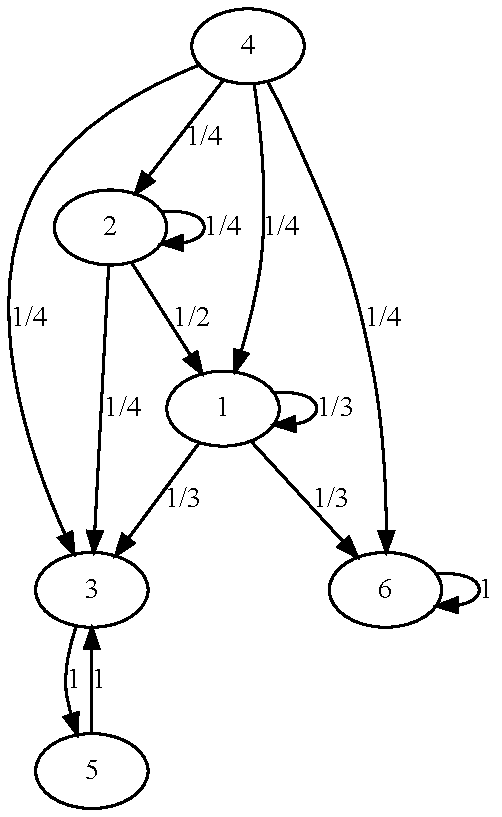
\includegraphics{Figure-24-04}
\end{figure}

States 3, 5, 6 are recurrent:

\begin{itemize}[tightlist]
\item
  A chain starting on state 6 will forever stay in state 6.
\item
  A chain starting on states 3 or 5 will bounce between states 3 and 5
  forever.
\end{itemize}

Other states are not recurrent, as they may eventually fall into state 6
and never reach other state after.

\textbf{Exercise 24.6.9}. Let

\[ P = \begin{bmatrix}
0 & 1 \\
1 & 0
\end{bmatrix}\]

Show that \(\pi = (1/2, 1/2)\) is a stationary distribution. Does this
chain converge? Why / why not?

\textbf{Solution}. The distribution is stationary if and only if
\(\pi = \pi P\), and

\[ \pi P = \begin{bmatrix} 1/2 & 1/2 \end{bmatrix}
\begin{bmatrix} 0 & 1 \\ 1 & 0 \end{bmatrix}
= \begin{bmatrix} 1/2 & 1/2 \end{bmatrix} = \pi
\]

This chain does not converge: it will always oscillate between states 1
and 2 with probability 1.

\textbf{Exercise 24.6.10}. Let \(0 < p < 1\) and \(q = 1 - p\). Let

\[ P = 
\begin{bmatrix}
q & p & 0 & 0 & 0 \\
q & 0 & p & 0 & 0 \\
q & 0 & 0 & p & 0 \\
q & 0 & 0 & 0 & p \\
1 & 0 & 0 & 0 & 0
\end{bmatrix}
\]

Find the limiting distribution of the chain.

\textbf{Solution}.

Solving \(\pi P = \pi\), we get:

\[ \pi = \begin{bmatrix} 
\frac{1 - p}{p^{4}(1 - p^{5})} &
\frac{1 - p}{p^{3}(1 - p^{5})} &
\frac{1 - p}{p^{2}(1 - p^{5})} &
\frac{1 - p}{p(1 - p^{5})} &
\frac{1 - p}{1 - p^{5}}
\end{bmatrix} \]

We can verify this is the limiting distribution:

\begin{align*}
\pi P &= \begin{bmatrix} \frac{1 - p}{p^{4}(1 - p^{5})} &
\frac{1 - p}{p^{3}(1 - p^{5})} &
\frac{1 - p}{p^{2}(1 - p^{5})} &
\frac{1 - p}{p(1 - p^{5})} &
\frac{1 - p}{1 - p^{5}}
\end{bmatrix}
\begin{bmatrix}
1 - p & p & 0 & 0 & 0 \\
1 - p & 0 & p & 0 & 0 \\
1 - p & 0 & 0 & p & 0 \\
1 - p & 0 & 0 & 0 & p \\
1 & 0 & 0 & 0 & 0
\end{bmatrix} \\
&= \begin{bmatrix} 
\frac{(1 - p)^{2}}{p^{4}(1 - p^{5})}
+ \frac{(1 - p)^{2}}{p^{3}(1 - p^{5})}
+ \frac{(1 - p)^{2}}{p^{2}(1 - p^{5})}
+ \frac{(1 - p)^{2}}{p(1 - p^{5})}
+ \frac{1 - p}{1 - p^{5}} &
\frac{1 - p}{p^{3}(1 - p^{5})} &
\frac{1 - p}{p^{2}(1 - p^{5})} &
\frac{1 - p}{p(1 - p^{5})} &
\frac{1 - p}{1 - p^{5}}
\end{bmatrix} \\
&= \begin{bmatrix} 
\frac{(1 - p)^{2}(1 + p + p^{2} + p^{3}) + p^{4}(1 - p)}{p^{4}(1 - p^{5})} &
\frac{1 - p}{p^{3}(1 - p^{5})} &
\frac{1 - p}{p^{2}(1 - p^{5})} &
\frac{1 - p}{p(1 - p^{5})} &
\frac{1 - p}{1 - p^{5}}
\end{bmatrix} \\
&= \begin{bmatrix} 
\frac{1 - p}{p^{4}(1 - p^{5})} &
\frac{1 - p}{p^{3}(1 - p^{5})} &
\frac{1 - p}{p^{2}(1 - p^{5})} &
\frac{1 - p}{p(1 - p^{5})} &
\frac{1 - p}{1 - p^{5}}
\end{bmatrix} \\
&= \pi
\end{align*}

\textbf{Exercise 24.6.11}. Let \(X(t)\) be an inhomogeneous Poisson
process with intensity function \(\lambda(t) > 0\). Let
\(\Lambda(t) = \int_{0}^t \lambda(u) du\). Define \(Y(s) = X(t)\) where
\(s = \Lambda(t)\). Show that \(Y(s)\) is a homogeneous Poisson process
with intensity \(\lambda = 1\).

\textbf{Solution}.

We have: \(Y(s) = X(\Lambda^{-1}(s))\) and
\(X(t) \sim \text{Poisson}(\Lambda(t))\), so

\[Y(s) \sim \text{Poisson}(\Lambda(\Lambda^{-1}(s)) = \text{Poisson}(s) = \text{Poisson}(\lambda_Y \cdot s)\]

which is the desired result with \(\lambda_Y = 1\).

\textbf{Exercise 24.6.12}. Let \(X(t)\) be a Poisson process with
intensity \(\lambda\). Find the conditional distribution of \(X(t)\)
given that \(X(t + s) = n\).

\textbf{Solution}. The random variables \(X(t) - X(0) = X(t)\) and
\(Y(s) = X(t + s) - X(t)\) are independent, as they are both count
increments, with \(X(t) \sim \text{Poisson}(\lambda t)\) and
\(Y(s) \sim \text{Poisson}(\lambda s)\). Then:

\begin{align*}
\mathbb{P}\left(X(t) = x | X(t + s) = n\right) &= \mathbb{P}\left(X(t) = x | X(t) + Y(s) = n\right) \\
&= \frac{\mathbb{P}\left(X(t) = x, X(t) + Y(s) = n\right)}{\mathbb{P}\left(X(t) + Y(s) = n\right)} \\
&= \frac{\mathbb{P}\left(X(t) = x, Y(s) = n - x\right)}{\sum_{0 \leq j \leq n} \mathbb{P}\left(X(t) = j, Y(s) = n - j\right)} \\
&= \frac{\mathbb{P}\left(X(t) = x\right) \mathbb{P}\left(Y(s) = n - x\right)}{\sum_{j=0}^{n} \mathbb{P}\left(X(t) = j\right) \mathbb{P}\left( Y(s) = n - j\right)} \\
&= \frac{f(x)}{\sum_{j=0}^{n} f(j) }
\end{align*}

where
\(f(x) = \mathbb{P}\left(X(t) = x\right) \mathbb{P}\left( Y(s) = n - x\right)\).
But we have:

\[ f(x) = \frac{(\lambda t)^x e^{-\lambda t}}{x!}\frac{(\lambda s)^{n - x} e^{-\lambda s}}{(n - x)!} = \frac{\lambda^{n} e^{-\lambda (t + s)}}{n!} \binom{n}{x} t^x s^{n - x} \]

Replacing on the expression above and cancelling the factors that do not
depend on \(x\), we get

\[ \mathbb{P}\left(X(t) = x | X(t + s) = n\right) = \frac{f(x)}{\sum_{j=0}^{n} f(j) } = \frac{\binom{n}{x} t^x s^{n - x}}{\sum_{j=0}^{n} \binom{n}{j} t^{j} s^{n - j}} 
= \frac{\binom{n}{x} t^x s^{n - x}}{(t + s)^{n}} = \binom{n}{x} \left( \frac{t}{t + s} \right)^x \left( \frac{s}{t + s}\right)^{n - x}\]

using the binomial expansion
\((t + s)^{n} = \sum_{j=0}^{n} \binom{n}{j} t^{j} s^{n - j}\). Therefore, the
conditional distribution follows a Binomial distribution,

\[ X(t) | X(t + s) = n \sim \text{Binomial}\left(n, \frac{t}{t + s} \right)\]

\textbf{Exercise 24.6.13}. Let \(X\) be a Poisson process with intensity
\(\lambda\). Find the probability that \(X(t)\) is odd,
i.e.~\(\mathbb{P}(X(t) = 1, 3, 5, \dots)\).

\textbf{Solution}. Expanding using the probability mass function,

\[
\mathbb{P}(X(t) \text{ is odd}) = \sum_{k=0}^{\infty} \frac{(\lambda t)^{2k + 1} e^{-\lambda t}}{(2k + 1)!} = e^{-\lambda t} \text{sinh} (\lambda t) = \frac{1}{2}\left( 1 - e^{-2 \lambda t}\right)
\]

\textbf{Exercise 24.6.14}. Suppose that people logging in to the
University computer system is described by a Poisson process \(X(t)\)
with intensity \(\lambda\). Assume that a person stays logged in for
some random time with CDF \(G\). Assume these times are all independent.
Let \(Y(t)\) be the number of people on the system at time \(t\). Find
the distribution of \(Y(t)\).

\textbf{Solution}.

The number of people arriving at time period \(j\) is
\(A(j) \equiv X(j) - X(j-1)\), where \(X(0) = 0\). Let \(W_{i}^{(j)}\) be
the amount of time spent by the \(i\)-th person that arrived at time
\(j\). Then, the total number of people at time \(t\) is:

\[ Y(t) = \sum_{j=1}^t \sum_{i=1}^{A(j)} I\left(W_{i}^{(j)} \geq t - j\right) \]

where \(I(x) = 1\) if \(x\) is true and \(0\) otherwise, and the terms
count only the people who are still logged in after an extra time
\(t - j\) elapsed.

Each value \(I\left(W_{i}^{(j)} \geq x\right)\) follows a distribution
given by \(1 - G(x)\), measuring the probability of a person staying
longer than time \(x\), and they are all independent.

We can write the sum above as:

\[ Y(t) = \sum_{j=1}^t B(j), \quad B(j) =\sum_{i = 1}^{A(j)} I\left(W_{i}^{(j)} \geq t - j\right) \]

Note that this implies that \(B(j) | A(j) = n\) follows a binomial
distribution with parameters \(n\) and
\(\mathbb{P}\left(W_{i}^{(j)} \geq t - j \right) = 1 - G(t - j)\).

Since \(A(j) \sim \text{Poisson}(\lambda)\) and
\(B(j) | A(j) = n \sim \text{Binomial}(n, 1 - G(t - j))\), the marginal
distribution of \(B(j)\) is
\(B(j) \sim \text{Poisson}\left(\lambda (1 - G(t - j))\right)\).
Therefore, \(Y\) being the sum of independent Poisson variables
\(B(j)\), we get that \(Y\) is a Poisson process with inhomogeneous rate
\(\lambda_Y(t)\),

\[ Y(t) \sim \text{Poisson}\left( \lambda_Y(t) \right), \quad \lambda_Y(t) = \lambda \left[ \sum_{j=1}^t(1 - G(t - j)) \right]\]

\textbf{Exercise 24.6.15}. Let \(X(t)\) be a Poisson process with
intensity \(\lambda\). Let \(W_{1}, W_{2}, \dots\) be the waiting times. Let
\(f\) be an arbitrary function. Show that

\[ \mathbb{E} \left[ \sum_{i=1}^{X(t)} f(W_{i}) \right] = \lambda \int_{0}^t f(w) dw \]

\textbf{Solution}.

When conditioning on \(X(t) = n\), the waiting times are uniformly
distributed on the interval \([0, t]\), so \(\sum_{i=1}^{n} f(W_{i})\) has
the same distribution as \(\sum_{i=1}^{n} f\left(U_{i}^{(n)}\right)\), for
\(U_{i}^{(n)} \sim \text{Uniform}(0, t)\). Then the expectation of
\(f\left(U_{i}^{(n)}\right)\) is

\[\mathbb{E}\left[ f\left(U_{i}^{(n)}\right) \right] = \int_{0}^t f(w) f_{U_{i}^{(n)}}(w) dw = \frac{1}{t} \int_{0}^t f(w) dw\]

Then, we have:

\begin{align*}
\mathbb{E}\left[ \sum_{i=1}^{X(t)} f(W_{i}) \right] 
&= \sum_{n = 0}^{\infty} \mathbb{E}\left[ \sum_{i=1}^{X(t)} f(W_{i}) \; \Bigg| \; X(t) = n\right] \mathbb{P} \left[ X(t) = n \right] \\
&= \sum_{n = 0}^{\infty} \mathbb{E}\left[ \sum_{i=1}^{n} f\left(U_{i}^{(n)}\right) \right] \mathbb{P} \left[ X(t) = n \right] \\
&= \sum_{n = 0}^{\infty} \frac{n}{t} \left( \int_{0}^t f(w) dw \right) \mathbb{P} \left[ X(t) = n \right] \\
&= \frac{1}{t} \left( \int_{0}^t f(w) dw \right) \sum_{n=0}^{\infty} n \; \mathbb{P} \left[ X(t) = n \right] \\
&= \frac{1}{t} \left( \int_{0}^t f(w) dw \right) \mathbb{E} \left[ X(t) \right] \\
&= \frac{1}{t} \left( \int_{0}^t f(w) dw \right) \lambda t \\
&= \lambda \int_{0}^t f(w) dw
\end{align*}

\textbf{Exercise 24.6.16}. A two dimensional Poisson process is a
process of random points in the plane such that (i) for any set \(A\),
the number of points falling in \(A\) is Poisson with mean
\(\lambda \mu(A)\) where \(\mu(A)\) is the area of \(A\), (ii) the
number of points in nonoverlapping regions is independent. Consider an
arbitrary point \(x_{0}\) in the plane. Let \(X\) denote the distance from
\(x_{0}\) to the nearest point. Show that

\[ \mathbb{P}(X > t) = e^{-\lambda \pi t^{2}} \]

and

\[ \mathbb{E}(X) = \frac{1}{2 \sqrt{\lambda}} \]

\textbf{Solution}. The distance \(X\) from \(x_{0}\) to the nearest point
is at least \(t\) if and only if no points lie within a circle of radius
\(t\) centered in \(x_{0}\). This circle \(C\) has area
\(\mu(C) = \pi t^{2}\), and so

\[ \mathbb{P}(X > t) = \mathbb{P}(\# \{\text{points in C} \} = 0) = f_C(0) = \frac{\lambda_C^{0} e^{-\lambda_C}}{0!} = e^{-\lambda_C} = e^{-\lambda \pi t^{2}} \]

Given that \(X\) has a CDF of \(F_X(x) = 1 - e^{-\lambda \pi x^{2}}\) for
\(x \geq 0\), its PDF is
\(f_X(x) = 2 \lambda \pi x e^{-\lambda \pi x^{2}}\), and its mean is

\[ \mathbb{E}(X) = \int_{0}^{\infty} x f_X(x) \; dx  = \int_{0}^{\infty} 2 \lambda \pi x^{2} e^{-2 \lambda \pi x^{2}} \; dx = \frac{1}{2 \sqrt{\lambda}}\]
